% !TEX root = ../intro-stellar-physics.tex

\section{Introduction: Our Sun}

Let's start by considering the star we know best: the Sun.  We'll denote the Sun with the symbol $\sun$. Measurements of the Earth-Sun distance have been done since antiquity\sidenote{For an account of how this was done, see \citet{Weinberg2015To-Explain-the-}.}. Observations of the planets' orbital periods, when combined with Kepler's laws, determine the planets' relative distances from the Sun. The distance scale is then fixed using radar ranging of objects in the solar system, with the mean Earth-Sun distance, known as an \newterm{astronomical unit}, being
\[
	\val{1}{\AU} = \val{\sci{1.5}{11}}{\meter}.
\]
From the orbits of the planets we can then deduce the mass\sidenote{Note that $G\Msun$ is known much more precisely than $G$ or $\Msun$ separately.} of the Sun:
\marginnote{Astronomy in the US uses the CGS system of units, whereas physics tends to use MKS. In these notes I follow the lead of undergraduate physics texts and also use MKS.}
\[
	\Msun = \val{\sci{1.99}{30}}{\kilo\gram}.
\]
The Sun is roughly $10^{6}$ times more massive than the Earth and 1\,000 times more massive than Jupiter.
The Sun subtends an angle of about $0.5^{\circ}$ across its diameter. Knowing the Earth-Sun distance and the angular size of the sun then tells us its radius:
\[
	\Rsun = \val{\sci{6.96}{8}}{\meter}.
\]
The total radiant power emitted by a star is its
\newterm{luminosity} $L$. A detector with a collecting area $\mathcal{A}$ located a distance $d$ from a star intercepts a fraction $\mathcal{A}/(4\pi d^{2})$ of the star's light.  We call $F = L/(4\pi d^{2})$ the \newterm{flux}, which has units $\watt\,\meter^{-2}$. 
Knowing the mean solar flux at \val{1}{\AU} allows us to infer the Sun's luminosity:
\[
	\Lsun = \val{\sci{3.86}{26}}{\watt}.
\]

\begin{exercisebox}[Solar power]
Suppose we wish to replace the MSU power plant---rated at $\val{70}{\Mega\watt}$ ($\val{\sci{70}{6}}{\watt}$)---with a grid of solar panels. Under ideal conditions (direct light and 100\% efficient panels), how many square meters of solar panels are needed?
\end{exercisebox}

\begin{exercisebox}[Flux from a distant star]
What would the flux be from a star with $L = \val{0.1}{\Lsun}$ at a distance of $\val{10}{\parsec}$?
Recall that a parsec (pc) is defined by the relation
\[
	\frac{\val{1}{\AU}}{\val{1}{\parsec}} = 1'' = \frac{1}{206\,265}.
\]
\end{exercisebox}

\section{Intensity and specific flux}
\label{s.intensity-specific-flux}

\begin{marginfigure}
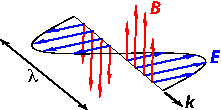
\includegraphics[width=\linewidth]{E-B-free-space}
\caption[The electric force in a light wave]{Schematic of the electric field (blue arrows) and magnetic field (red arrows) for a wave traveling along direction $\bvec{k}$ with wavelength $\lambda$.}
\label{f.light-wave}
\end{marginfigure}
When we detect light, what happens at the atomic level is that the charges in our detector (antenna, CCD, eye) feel an electric (and magnetic) force that oscillates with frequency $\nu$. Imagine setting up a grid of detectors that measure the electric and magnetic forces per charge at each point in space and at each instant of time. We call these forces per charge the electric and magnetic fields, $\bvec{E}(\bvec{x},t)$ and $\bvec{B}(\bvec{x},t)$. As light passes through this grid, we would notice a sinusoidal pattern traveling at speed\sidenote{This velocity is exact; the meter is defined in terms of the speed of light.} $c = \val{299\,792\,458}{\meter/\second}$ with a wavelength $\lambda = c/\nu$.  The amplitude of the light at our detector is proportional to $|\bvec{E}|^{2} + |\bvec{B}|^{2}$. 

Suppose we put a filter in front of our detector that only accepted light in a narrow range of wavelengths $(\lambda,\lambda+\Delta\lambda)$. We would find that energy is deposited into our detector in discrete quanta, known as \newterm{photons}, with each photon having an energy $hc/\lambda = h\nu$\marginnote{The symbol $h = \val{\sci{6.63}{-34}}{\unitstyle{J}\usk\second}$ denotes \newterm{Planck's constant}.}. The light emitted by the Sun (or any other source) consists of a huge number of photons distributed over a broad range of wavelengths, known as a \newterm{spectrum}.

\begin{exercisebox}[Photon flux from the sun]
The peak of the sun's spectrum is at a wavelength of approximately $\val{500}{\nano\meter}$. Estimate the number of photons from the sun striking $\val{1}{\meter^{2}}$ of Earth each second.
\end{exercisebox}

\begin{marginfigure}[6\baselineskip]
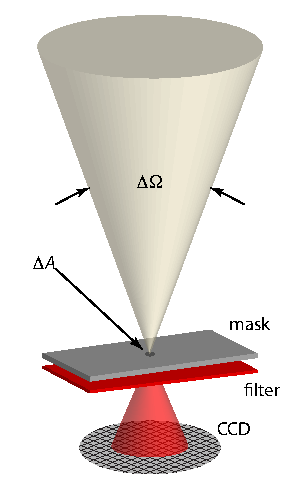
\includegraphics[width=\linewidth]{intensity}
\caption{\label{f.intensity} Schematic of radiative intensity}
\end{marginfigure}
Take a detector (a CCD, an eye, a photographic emulsion) and place (see Fig.~\ref{f.intensity}) in front of the detector a filter that only lets through light with wavelengths in a range $\Delta\lambda$. Place a mask over the detector with a small pinhole of area $\Delta A$ that restricts the light falling on the detector to fall in a narrow cone of solid angle $\Delta\Omega$ about the normal to the detector. Then measure the energy $\Delta E$ incident on the detector in a time $\Delta t$. The quantity
\begin{equation}\label{e.definition-intensity}
I_{\lambda} \equiv \frac{\Delta E}{\Delta t\,\Delta A\,\Delta\lambda\,\Delta\Omega}
\end{equation}
is known as the \newterm{intensity}. It is the basic quantity describing radiation.

In situations in which the wavelength is small (relative to the system in question so we can neglect diffraction), light propagates along \newterm{rays}. By a ray of light, we mean the light emitted into a small cone of opening solid angle $\dif\Omega$ about a direction $\unitk$. In the absence of any interactions with matter, the intensity is conserved along a ray if both source and receiver are stationary with respect to one another (Exercise~\ref{ex.intensity-conserved}).

\begin{sidebar}[Solid angles]
\label{sb.solid-angles}
Imagine that your are at the center of a great sphere of radius $R$, and you shine a light that emits rays into some solid angle. Orient your coordinates so that the rays are traveling along the $z$-axis. The light will illuminate an area
\[ 	A = R^{2}\int_{0}^{2\pi}\int_{0}^{\theta}\sin\theta\,\dif\theta\,\dif\phi. \]
Here $\theta$ is the opening half-angle of the cone. The solid angle into which the light is emitted is $\Omega = A/R^{2}$. Astronomers often express the integral by changing variables to $\mu = \cos\theta$, so that the solid angle is
\[
	\Delta\Omega = \int_{0}^{2\pi}\int_{1-\Delta\mu}^{1}\dif\mu\,\dif\phi.
\]
If we integrate over all angles ($0\le\theta\le\pi$, or $-1\le\mu\le 1$), then we get the area of a sphere, $A = 4\pi R^{2}$.
\end{sidebar}

\begin{exercisebox}[Proof that $I_{\lambda}$ is conserved]
\label{ex.intensity-conserved}
Your friend flashes a light: in a time $\Delta t$ it emits a energy $\Delta E_{\mathrm{emit}}$ in a waveband $\Delta\lambda$. The opening through which the light passes has area $\Delta A_{\mathrm{emit}}$, and the light goes into a cone of opening solid angle $\Delta\Omega_{\mathrm{emit}}$ (see Fig.~\ref{f.intensity-conserved}). Your friend therefore calculates her intensity as
\[	
	I_{\lambda,\mathrm{emit}} = \frac{\Delta E_{\mathrm{emit}}}{\Delta t\,\Delta A_{\mathrm{emit}}\,\Delta\lambda \,\Delta\Omega_{\mathrm{emit}}}.
\]
You stand a distance $d$ ($d^{2}\gg \Delta A_{\mathrm{emit}}, \Delta A_{\mathrm{obs}}$) from your friend with a camera. The aperture on your camera has area $\Delta A_{\mathrm{obs.}}$. Show that the intensity you receive is $I_{\lambda,\mathrm{obs}} = I_{\lambda,\mathrm{emit}}$.
\begin{enumerate}
\item Calculate the incident energy that falls on your camera aperture $\Delta E_{\mathrm{obs}}$.
\item What solid angle $\Delta\Omega_{\mathrm{obs}}$ is subtended by the rays entering the aperture?
\item Now compute your intensity
\[	
	I_{\lambda,\mathrm{obs}} = \frac{\Delta E_{\mathrm{obs}}}{\Delta t\,\Delta A_{\mathrm{obs}}\,\Delta\lambda \,\Delta\Omega_{\mathrm{obs}}}.
\]
and show that this is the same as what your friend calculated.
\end{enumerate}
\end{exercisebox}
\begin{figure*}
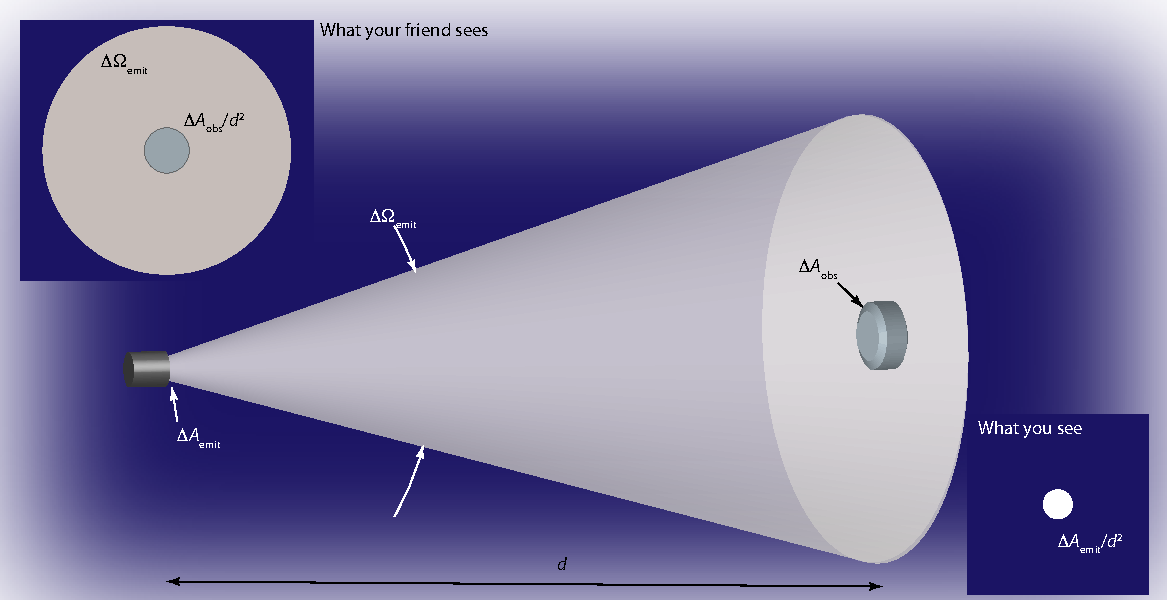
\includegraphics[width=\linewidth]{intensity-conserved}
\caption[Schematic of intensity being constant]{\label{f.intensity-conserved} Schematic for exercise \ref{ex.intensity-conserved}.}
\end{figure*}

To compute the \newterm{specific flux} $F_{\lambda}$, we multiply the intensity by $\cos\theta$, where $\theta$ is the angle between the ray and the normal of our area\sidenote{this gives the projected area} and integrate over angle:
\begin{equation}\label{e.specific-flux}
F_{\lambda} =  \int I_{\lambda}\,\cos\theta\,\sin\theta\,\dif\theta\,\dif\phi.
\end{equation}
The specific flux has dimensions
\[
	[F_{\lambda}] \sim \frac{\textrm{energy}}{\textrm{time}\cdot\textrm{area}\cdot\textrm{wavelength}}.
\]


\section{Thermal emission}
\label{s.thermal-emission}

Imagine we had a material that emits and absorbs equally well at all wavelengths. We then made from this material a hollow box, and we heated this box to a temperature $T$. The hot atoms in the walls of the box would emit (and absorb) photons bouncing around in the cavity in this box, until the photons were in thermal equilibrium\sidenote{Meaning that the radiation field is on average neither gaining or losing energy from the walls of the box} with the walls of the box. If we then drilled a small hole in the side of the box, some photons would escape (but not so many as to disturb the thermal equilibrium). The intensity emerging from such a box is known as the \newterm{Planck spectrum}:
\begin{equation}\label{e.planck-spectrum-wavelength}
I_{\lambda}(\mathrm{Planck}) \equiv B_{\lambda}(T) = \frac{2hc^{2}}{\lambda^{5}} \left[\exp\left(\frac{hc}{\lambda\kB T}\right)-1\right]^{-1}.
\end{equation}
Here $\kB = \val{\sci{1.381}{-23}}{\unitstyle{J}\usk\K^{-1}}$ denotes \newterm{Boltzmann's constant}. This spectrum is also known as a \newterm{blackbody} spectrum, because it is emitted from a material that absorbs (and therefore emits) equally well at all wavelengths. The emission is peaked at a wavelength $\lambda_{\mathrm{pk}} \sim hc/\kB T$. 
Fig.~\ref{f.Planck} displays Planck's spectra for various temperatures. Note that $B_{\lambda}$ increases at all wavelengths as the temperature increases.
\begin{marginfigure}
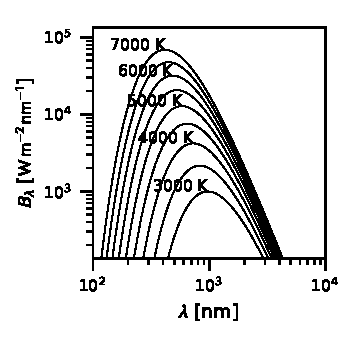
\includegraphics[width=\linewidth]{Planck}
\caption[Thermal spectra]{\label{f.Planck}Thermal spectra for temperatures ranging from \val{3000}{\K} to \val{7000}{\K}.}
\end{marginfigure}

\begin{exercisebox}[Peak of thermal spectrum]\label{ex.Wien-wavelength}
Show that the peak of the thermal spectrum, temperature $T$, occurs (i.e., where $B_{\lambda}$ is maximum) at a wavelength
\[ \lambda_{\mathrm{pk}} = \val{290}{\nano\meter}\left(\frac{\val{10\,000}{\K}}{T}\right). \]
This result is known as \newterm{Wien's law}. Check this: what is the peak wavelength of the sun's emission? What is the peak wavelength for the cosmic microwave background ($T_{\mathrm{CMB}} = \val{2.73}{\K}$)?
\end{exercisebox}

The Planck spectrum, expressed in terms of frequency, is
\begin{equation}\label{e.planck-spectrum-frequency}
B_{\nu}(T) = \frac{2h\nu^{3}}{c^{2}} \left[\exp\left(\frac{h\nu}{\kB T}\right)-1\right]^{-1}.
\end{equation}

\begin{exercisebox}[Frequency peak in thermal spectrum]
What is the frequency corresponding to $\lambda_{\mathrm{pk}}$ in Exercise~\ref{ex.Wien-wavelength}? Compute the frequency $\nu_{\mathrm{pk}}$ at which $B_{\nu}$ is maximum. Is $\nu_{\mathrm{pk}}$ the same as the frequency corresponding to $\lambda_{\mathrm{pk}}$?
\end{exercisebox}

Suppose we try to compute the specific flux using Eq.~(\ref{e.specific-flux}). Since $B_{\lambda}$ doesn't depend on angle, the integral is easy:
\[ F_{\lambda} = B_{\lambda}\int_{0}^{2\pi}\int_{0}^{\pi}\cos\theta\,\sin\theta\,\dif\theta\,\dif\phi = 0. \]

\begin{exercisebox}[No net flux for thermal emission]
Explain, without using mathematical expressions, why there is no net flux for thermal emission.
\end{exercisebox}

Although the net flux is zero, if we just want the radiation escaping from our cavity, we only want to integrate over the angles $0\le\theta\le\pi/2$. If we do this, then our \emph{outward-going} specific flux is
\begin{equation}\label{e.outward-thermal-flux}
 F_{\lambda}(\mathrm{outward}) = B_{\lambda}\int_{0}^{2\pi}\int_{0}^{\pi/2}\cos\theta\,\sin\theta\,\dif\theta\,\dif\phi = \pi B_{\lambda}.
\end{equation}
To find the total power emitted per area for thermal radiation, we need to integrate $F_{\lambda}$ over wavelength:
\begin{equation}\label{e.bolometric-thermal-flux}
F = \int_{0}^{\infty}F_{\lambda}(\mathrm{outward})\,\dif\lambda 
	= \int_{0}^{\infty} \frac{2\pi hc^{2}}{\lambda^{5}} \frac{\dif\lambda}{\exp\left(hc/\lambda\kB T\right)-1}.
\end{equation}
By changing variables to $x = hc/\lambda\kB T$, we can write this integral as\marginnote{The integral over $x$ can be converted into a Riemann zeta function; for further information, consult a text on mathematical methods in physics.}
\[
	F = \frac{2\pi\kB^{4}}{h^{2}c}T^{4}\times \underbrace{\int_{0}^{\infty}\frac{x^{3}}{e^{x}-1}\,\dif x}_{=\pi^{4}/15} = \left[\frac{2\pi^{5}}{15}\frac{\kB^{4}}{h^{2}c}\right] T^{4}.
\]
The quantity in $\left[\cdot\right]$ is called the \newterm{Stefan-Boltzmann constant}:
\[
	\sigmaSB = \val{\sci{5.7}{-8}}{\watt\usk\meter^{-2}\usk\K^{-4}};
\]
The total energy radiated per second per area from a thermal emitter of temperature $T$ is thus $\sigmaSB T^{4}$.

\newthought{Real stars are \emph{not} blackbodies!} That being said, their spectra are roughly thermal, so we can define an \newterm{effective surface temperature}
\[	\Teff = \left[\frac{F}{\sigmaSB}\right]^{1/4}. \]
The total power output, or \emph{luminosity}, of a star of radius $R$ is thus
\[
	L = 4\pi R^{2}\sigmaSB \Teff^{4}.
\]
For the sun, $\Teff = \val{5780}{\K}$.


\section{The radiation energy density}\label{s.radiation-energy-density}

We introduced
\[
I_{\lambda} \equiv \frac{\dif E}{\dif t\,\dif A\,\dif\lambda\,\dif\Omega}
\]
as the radiant energy $\dif E$ crossing an area $\dif A$ in a time $\dif t$, directed into a solid angle $\dif\Omega$, and carried by photons with wavelengths in a range $\dif\lambda$. Notice that in time $\dif t$, these photons will fill a volume $\dif V = c\dif t\times \dif A$. Hence we can write the intensity as
\[
I_{\lambda} = c\frac{\dif E}{\dif V\,\dif \lambda\,\dif\Omega}.
\]
Using this expressions, we define the radiant energy density per wavelength as
\begin{equation}
	U_{\lambda} \equiv \frac{\dif E}{\dif V\,\dif\lambda} = \frac{1}{c}\int I_{\lambda}\,\dif \Omega.
\end{equation}
If the radiation is thermal, that is, if $I_{\lambda} = B_{\lambda}$, then
\[
U_{\lambda} = \frac{B_{\lambda}}{c}\int_{0}^{2\pi}\int_{0}^{\pi}\sin\theta\,\dif\theta\,\dif\phi = \frac{4\pi}{c}B_{\lambda},
\]
and the total radiant energy density is
\[
U = \int_{0}^{\infty}U_{\lambda}\,\dif\lambda = \frac{4}{c}\pi\int_{0}^{\infty}B_{\lambda}\,\dif\lambda = \left[\frac{4\sigmaSB}{c}\right] T^{4}.
\]
In this expression, 
\[ 
a = \left[\frac{4\sigmaSB}{c}\right] = \val{\sci{7.566}{-16}}{\unitstyle{J}\usk\meter^{-3}\usk\K^{-4}}.
\]
and we have used equations~(\ref{e.outward-thermal-flux}) and (\ref{e.bolometric-thermal-flux}). The energy density of thermal radiation is $U = aT^{4}$.

It is common to denote the average (over angle) intensity as
\begin{equation}\label{e.angle-average-intensity}
J_{\lambda} = \frac{1}{4\pi}\int I_{\lambda}\,\dif\Omega;
\end{equation}
the specific energy density is thus
\[ U_{\lambda} = \frac{4\pi}{c}J_{\lambda}. \]

\begin{sidebar}[Momentum transport and radiation pressure]
\label{sb.radiation-pressure}
In addition to transporting energy, photon also carry momentum. You will learn in your quantum mechanics course that the momentum of a photon of energy $h\nu$ traveling along direction $\unitk$ is
\[ \bvec{p} = \frac{h\nu}{c}\unitk = \frac{h}{\lambda}\unitk. \]
Here $\nu$ and $\lambda = c/\nu$ are the frequency and wavelength of the photon. Hence the momentum carried by photons of energy $E_{\nu}$ along direction $\unitk$ is $E/c$. Since $I_{\nu}$ is the amount of energy carried by photons per area per time along the direction $\unitk$, the momentum transported by those photons per area per time along direction $\unitk$ must be $(I_{\nu}/c)\unitk$.

\newthought{To relate this momentum transport to the radiation pressure,} suppose we have a sheet of absorbing material with a normal $\unitn$ being impinged by a ray of photon traveling along $\unitk$. As the photons are absorbed, they transfer momentum (along direction $\unitn$) of $(E_{\nu}/c)\unitn\vdot\unitk$ to the matter. The projected area of the ray on the matter is $\dif A\,\unitn\vdot\unitk$. The rate of momentum transfer along $\unitn$ per area per frequency is therefore
\begin{eqnarray}
P_{\!\nu} &=& \frac{1}{c}\int I_{\nu}
	{\color{red}\underbrace{\left(\unitn\vdot\unitk\right)}_{\textrm{proj.~area}}}
	{\color{blue}\underbrace{\left(\unitn\vdot\unitk\right)}_{\textrm{comp.\ of $\bvec{p}$ along $\unitn$}}}
	\,\dif\Omega \nonumber\\
	&=& \frac{1}{c}\int_{0}^{2\phi}\int_{-1}^{1}I_{\nu} \mu^{2}\,\dif \mu\,\dif\phi.
\label{e.momentum-transfer}
\end{eqnarray}
A change in momentum per time is a force; hence equation~(\ref{e.momentum-transfer}) represents the force per area, or \newterm{pressure}, exerted by photons with frequencies in $[\nu,\nu+\dif\nu]$. The two factors of $\mu=\cos\theta$ account for the projected area and the component of momentum along the normal to the surface $\unitn$.

If the radiation is thermal, so that $I_{\nu} = B_{\nu}$ and is independent of angle, then
\[
	P_{\!\nu} = \frac{4\pi}{3c}B_{\nu}.
\]
We can integrate $P_{\!\nu}$ over frequency to get the total radiation pressure,
\begin{equation}\label{e.radiation-pressure}
	\Prad = \frac{4\pi}{3c}\int_{0}^{\infty}B_{\nu}\,\dif\nu = \frac{4}{3c}\sigmaSB T^{4} = \frac{1}{3}aT^{4}.
\end{equation}
Note that the pressure is $1/3$ of the energy density for thermal radiation. This is in general true for a gas of relativistic particles that have momentum proportional to energy.
\end{sidebar}

\section{Magnitudes}
\label{s.magnitudes}

When observing a star, astronomers are collecting light over a range of frequencies. To compare observations, astronomers typically pass the light through standard filters and measure the transmitted flux. The flux in a given band is then
\[
	F_{\mathrm{band}} = \int F_{\lambda} \, T(\lambda)\,\dif\lambda.
\]
Here $T(\lambda)$ is the \newterm{transmission function} for that filter and specifies how much light is let through as a function of wavelength.  The transmission functions for some common UV/optical/IR filters are shown in Figure~\ref{f.UBVRI}. For example, the $V$-band filter is centered at $\lambda=\val{551}{\nano\meter}$ and has a width at half-max of $\val{88}{\nano\meter}$. 
\begin{figure}
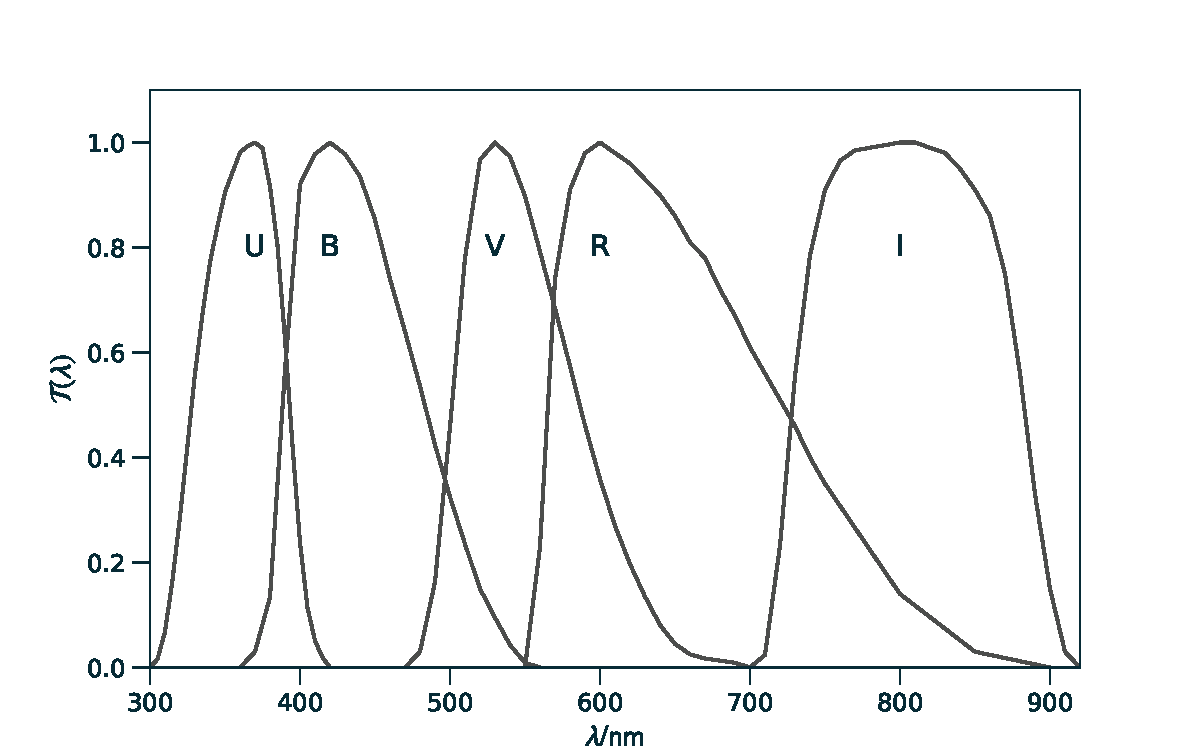
\includegraphics[width=\linewidth]{UBVRI}
\caption[Standard filters]{\label{f.UBVRI} Some standard UV/optical/IR filters. The $T(\lambda)$ are normalized so that $\max(T)=1$.}
\end{figure}

\begin{exercisebox}[Filter for observing sun-like star]
Suppose you wished to observe a sun-like star, and you wanted to observe wavelengths near the peak of the spectrum.  Which filter would you choose, and why?  What about for a star with a surface effective temperature $\Teff = \val{8\,000}{\K}$? 
\end{exercisebox}

When making observations, it is common to compare the fluxes in a particular band between two stars. Optical astronomers therefore define the \emph{apparent magnitude} as
\marginnote{NB. Throughout this text, $\log\equiv\lg$ denotes $\log_{10}$ and $\ln$ denotes $\log_{e}$.}
\begin{equation}\label{e.apparent-magnitude}
m(A) - m(B) = -2.5\log\left[\frac{F(A)}{F(B)}\right].
\end{equation}
Here $F(A)$ and $F(B)$ are two different measurements of flux (from two different stars, for example) in a particular waveband. It is common to use the label of the waveband in place of $m$. Thus, for example, when an astronomer says, ``The $V$-magnitude is 16.6'', what she means is that the apparent magnitude measured with a standard $V$-filter is 16.6.

As an application of this, imagine comparing the flux from a star, at a distance $d$, with that from an imaginary identical star located at a distance of $\val{10}{\parsec}$. We'll call the magnitude of this imaginary star at $\val{10}{\parsec}$ the \newterm{absolute magnitude} $M$ and define the \newterm{distance modulus} as
\begin{eqnarray}
\mathrm{DM} \equiv m-M &=& m(d) - m(\val{10}{\parsec})\nonumber\\
&=& -2.5\log\left[\frac{L/4\pi d^{2}}{L/4\pi(\val{10}{\parsec})^{2}}\right]\nonumber\\
&=& -2.5\log\left[\left(\frac{\val{10}{\parsec}}{d}\right)^{2}\right]\nonumber \\
&=& 5\log\left(\frac{d}{\parsec}\right) - 5.
\end{eqnarray}
Since the absolute magnitude is a measure of the flux from the star \emph{if it were} at a specified distance, the absolute magnitude is a proxy for the luminosity \emph{measured in a given filter}.

\newthought{We can also compare the flux from two different filters for the same star.} The difference in magnitudes for two different filters defines a \newterm{color index}, which is a measure of the star's spectrum (and, roughly, its temperature). For example,
\[
	B - V \equiv m_{B}-m_{V} = -2.5\log\left[\frac{\int_{B-\mathrm{band}}F_{\lambda}\,\dif\lambda}{\int_{V-\mathrm{band}}F_{\lambda}\,\dif\lambda}\right]
\]
measures the ratio of fluxes in the $B$ and $V$ bands for a particular star.

\begin{exercisebox}[Color index and temperature]
How would the $B-V$ index of the sun compare to that of a hotter star, e.g., one with $\Teff = \val{8\,000}{\K}$?
\end{exercisebox}

